\PassOptionsToPackage{export}{adjustbox}
\documentclass[
	11pt,
	aspectratio=169,
]{beamer}

\graphicspath{{supplement/}{./}}

\usepackage{booktabs}
\usepackage{multirow}
\usepackage{amsmath,amssymb,amsfonts}
\usepackage{algorithm}
\usepackage{algorithmic}
\usepackage{graphicx}
\usepackage{caption}
\usepackage{subcaption}
\usepackage{tikz}
\usetikzlibrary{shapes.geometric,arrows,positioning}
\usepackage{standalone}
\usepackage{colortbl}
\usepackage[export]{adjustbox} % For max width/height in includegraphics

% Global Image Constraints
\setkeys{Gin}{max width=0.9\textwidth, max height=0.75\textheight, keepaspectratio}

% Global List Spacing
\setbeamertemplate{itemize/enumerate body begin}{\small}
\setbeamertemplate{itemize/enumerate subbody begin}{\footnotesize}
\setlength{\leftmargini}{1.5em}
\setlength{\leftmarginii}{1.2em}
\setlength{\itemsep}{0.3em} 

% Theme
\usetheme{Boadilla}
\usecolortheme{seahorse}

% Custom Colors
\definecolor{mathblue}{RGB}{0,51,102}
\definecolor{mathgray}{RGB}{64,64,64}
\definecolor{lightgray}{RGB}{240,240,240}

\setbeamercolor{structure}{fg=mathblue}
\setbeamercolor{frametitle}{fg=mathblue,bg=white}
\setbeamercolor{title}{fg=mathblue}
\setbeamercolor{author}{fg=mathgray}

% Fonts
\usefonttheme{default}
\usepackage{palatino}
\usepackage[default]{opensans}

% Custom Frametitle
\let\oldframetitle\frametitle
\renewcommand{\frametitle}[1]{%
    \ifx\insertsection\empty%
        \oldframetitle{#1}%
    \else%
        \oldframetitle{%
            {\small\color{mathblue}\textbf{\thesection. \insertsection}}%
            \hspace{0.4em}{\color{gray!50}|}\hspace{0.4em}%
            #1%
        }%
    \fi%
}

\title[Accelerating the Sol...]{Accelerating the Solution of Linear Systems by Iterative Refinement in Three Precisions}
\subtitle{Generated by Paper2PPT (github.com/gejifeng/Paper2PPT)}
\author{Erin Carson and Nicholas J. Higham}
\date{\today}

\begin{document}\begin{frame}
	\titlepage
\end{frame}
\begin{frame}{Overview}
	\tableofcontents
\end{frame}



\section{Introduction}


\begin{frame}{Motivation}
    \begin{block}{The Problem}
Solving $A x = b$ for large systems is computationally expensive, dominated by the $O(n^3)$ factorization step.
\end{block}

\begin{itemize}
    \item Modern hardware (GPUs) supports faster, lower-precision arithmetic (e.g., half precision).
    \item Can we leverage this to accelerate linear solvers without losing accuracy?
\end{itemize}

\begin{block}{Key Idea: Mixed Precision}
Use different precisions for different parts of the computation:
\begin{itemize}
    \item \textbf{Low precision} for the expensive factorization ($u_f$).
    \item \textbf{High precision} for accurate residual calculations ($u_r$).
    \item \textbf{Working precision} for the final solution ($u$).
\end{itemize}
\end{block}
\end{frame}
\begin{frame}{The Three Precisions}
    \begin{block}{Four Precision Parameters}
The general framework uses four precisions:
\begin{itemize}
    \item \textbf{Working precision} $u$: Stores data $A$, $b$ and solution $x$.
    \item \textbf{Factorization precision} $u_f$: Computes the LU factorization.
    \item \textbf{Solver precision} $u_s$: Solves the correction equation $A d = r$.
    \item \textbf{Residual precision} $u_r$: Computes residuals $r = b - A x$.
\end{itemize}
\end{block}

\begin{block}{Required Precision Hierarchy}
For the algorithm to function correctly, the precisions must satisfy:
\begin{equation*}
u_r \leq u \leq u_f
\end{equation*}
Additionally, the solver precision is bounded by $u \leq u_s \leq u_f$.
\end{block}
\end{frame}
\begin{frame}{Existing Analyses}
    \begin{block}{Goal of This Work}
Develop a \textbf{unified analysis} of iterative refinement for linear systems.
\begin{itemize}
    \item Generalize existing analyses to three precisions.
    \item Cover new scenarios (e.g., half-precision factorization).
\end{itemize}
\end{block}

\begin{table}
\centering
\begin{tabular}{l l l l}
\toprule
\textbf{Study} & \textbf{Solver} & \textbf{Error Type} & \textbf{Precision Assumptions} \\
\midrule
Moler (1967) & LU & Normwise & $u_r \leq u$ \\
Skeel (1991) & Arbitrary & Componentwise & $u_r \leq u$ \\
Langou et al. (2006) & LU & Normwise & $u_r \leq u$ \\
\midrule
\textbf{This Work} & \textbf{Arbitrary} & \textbf{Both} & \textbf{General ($u_r \leq u \leq u_f$)} \\
\bottomrule
\end{tabular}
\end{table}
\end{frame}


\section{Background}


\begin{frame}{Preliminaries \& Notation}
\setlength{\itemsep}{0pt}
\begin{block}{Unit Roundoff}
The unit roundoff $u$ is the maximum relative error due to rounding:
\[
u = \frac{1}{2} \beta^{1-p}
\]
where $\beta$ is the base and $p$ is the precision.
\end{block}
\vspace{-0.5em}
\begin{block}{Auxiliary Quantities}
For integer $k$, define $\gamma_k = \frac{k u}{1 - k u}$. Superscripts denote precision, e.g., $\gamma_k^r = k u_r / (1 - k u_r)$.
\end{block}
\vspace{-0.5em}
\begin{block}{Condition Numbers}
\textbf{Normwise:} $\kappa_{\infty}(A) = \| A^{-1} \|_{\infty} \| A \|_{\infty}$ \\
\textbf{Componentwise:} $\text{cond}(A) = \parallel |A^{-1}| |A| \parallel_{\infty}$
\end{block}
\end{frame}
\begin{frame}{Solver Assumptions}
    \begin{alertblock}{Solver Assumptions}
The solver for the correction equation must be backward stable, satisfying three conditions for each computed correction $\widehat{d}_i$:
\end{alertblock}

\begin{block}{Equations (2.3)-(2.5)}
\begin{itemize}
    \item \textbf{Forward Error:} $\widehat{d}_i = (I + u_s E_i) d_i$ with $\|E_i\|_\infty < 1/u_s$
    \item \textbf{Normwise Backward Error:} $\| \widehat{r}_i - A\widehat{d}_i \|_\infty \leq u_s ( c_1 \|A\|_\infty \|\widehat{d}_i\|_\infty + c_2 \|\widehat{r}_i\|_\infty )$
    \item \textbf{Componentwise Backward Error:} $| \widehat{r}_i - A\widehat{d}_i | \leq u_s G_i | \widehat{d}_i |$
\end{itemize}
\end{block}
\end{frame}


\section{Methodology}


\begin{frame}{General Algorithm}
    \begin{block}{Algorithm 1.1: Iterative Refinement}
Given $A \in \mathbb{R}^{n \times n}$ and $b \in \mathbb{R}^{n}$ in precision $u$.
\begin{enumerate}
    \item Compute initial guess $x_0$ in precision $u_f$.
    \item \textbf{for} $i = 0, 1, \dots$
    \item Compute residual $r_i = b - A x_i$ in precision $u_r$.
    \item Solve correction equation $A d_i = r_i$ in precision $u_s$.
    \item Update solution $x_{i+1} = x_i + d_i$ in precision $u$.
    \item \textbf{end for}
\end{enumerate}
\end{block}

\begin{itemize}
    \item \textbf{Key Insight:} Decouples precisions for storage ($u$), solver ($u_f, u_s$), and residuals ($u_r$).
    \item \textbf{Flexibility:} The solver in step 1 (factorization) can differ from step 4 (correction).
    \item \textbf{Goal:} Perform expensive $O(n^3)$ work in low precision (e.g., half).
    \item \textbf{Result:} Achieves high precision (e.g., single) accuracy using low precision solvers.
\end{itemize}
\end{frame}
\begin{frame}{Forward Error Analysis}
    \begin{block}{Theorem 3.2: Forward Error Bound}
The forward error after iteration $i$ satisfies
\begin{equation*}
\frac{\|x_i - \widehat{x}_i\|_\infty}{\|x_i\|_\infty} \leq \eta_i,
\end{equation*}
where $\eta_i$ evolves according to the recurrence
\begin{equation*}
\eta_{i+1} \leq \theta \eta_i + \beta \eta_i^2.
\end{equation*}
\end{block}

\begin{itemize}
    \item $\theta$ depends on the solver accuracy $u_s$ and condition numbers.
    \item $\beta$ depends on the residual precision $u_r$ and the condition number.
    \item Convergence requires $\theta < 1$.
\end{itemize}
\end{frame}
\begin{frame}{Convergence \& Accuracy}
    \begin{block}{Corollary 3.3 (Convergence \& Accuracy)}
The convergence rate of Algorithm 1.1 depends on the solver precision $u_s$, while the final forward error is bounded by a function of the residual precision $u_r$ and the working precision $u$.
\end{block}

\begin{itemize}
    \item \textbf{Convergence Rate}: Determined by $u_s$.
    \item \textbf{Final Accuracy}: Determined by $u_r$ and $u$.
    \item \textbf{Key Insight}: High precision residuals ($u_r \ll u$) enable high final accuracy.
    \item \textbf{Solver Precision}: $u_s$ must be $\geq u$ for convergence.
\end{itemize}
\end{frame}
\begin{frame}{Backward Error Analysis}
    \begin{columns}[T,onlytextwidth]
    \begin{column}{0.48\textwidth}
        \begin{block}{Normwise Backward Error (Theorem 4.1)}
        The backward error $\eta(\hat{x})$ satisfies:
        \begin{equation*}
        \eta(\hat{x}) \leq \frac{c_1 u_f + c_2 u_r}{1 - \kappa_\infty(A) u_s}
        \end{equation*}
        \end{block}
        \begin{itemize}
            \item Requires $\kappa_\infty(A) u_s < 1$.
            \item Iterative refinement restores stability if solver is stable.
            \item High condition numbers limit accuracy.
        \end{itemize}
    \end{column}
    \begin{column}{0.48\textwidth}
        \begin{block}{Componentwise Backward Error (Theorem 5.1)}
        The backward error $\omega(\hat{x})$ satisfies:
        \begin{equation*}
        \omega(\hat{x}) \approx \frac{\|G\|_\infty u_f + u_r}{1 - \text{cond}(A) u_s}
        \end{equation*}
        \end{block}
        \begin{itemize}
            \item Uses componentwise condition number $\text{cond}(A)$.
            \item Allows accurate solutions for ill-conditioned $A$.
            \item GMRES-IR extends solvable range.
        \end{itemize}
    \end{column}
\end{columns}
\end{frame}
\begin{frame}{Scaling}
    \begin{block}{The Need for Scaling}
When using low precision (e.g., half) for the solve step, values can easily exceed the representable range.
\end{block}

\begin{itemize}
    \item The correction $d_i$ can be large if the residual $r_i$ is large.
    \item This leads to \textbf{overflow} or \textbf{underflow} in the solver.
    \item Scaling the system $A d = r$ prevents numerical exceptions.
\end{itemize}

\begin{alertblock}{Visual Placeholder}
Diagram showing the iterative refinement loop with a scaling step before the low-precision solver.
\end{alertblock}
\end{frame}


\section{Experiments}


\begin{frame}{LU Factorization Scenarios}
    \begin{block}{LU Factorization Scenarios}
Three main scenarios for iterative refinement with LU factorization are analyzed:
\begin{itemize}
    \item \textbf{Traditional}: Residuals in double precision, solver in single precision.
    \item \textbf{Fixed Precision}: All computations (solver, residuals) in single precision.
    \item \textbf{Mixed Precision (New)}: Solver in half precision, residuals in double precision.
\end{itemize}
\end{block}

\begin{itemize}
    \item The new method performs the $O(n^3)$ factorization entirely in half precision.
    \item This achieves full single precision accuracy for $\kappa_{\infty}(A) \leq 10^4$.
    \item Speedups of up to 2x are possible on hardware with efficient half precision.
\end{itemize}
\end{frame}
\begin{frame}{New Results: Half Precision}
    \begin{alertblock}{Key Finding}
Solving to single precision accuracy is possible for condition numbers up to $\kappa_{\infty}(A) \leq 10^4$.
\end{alertblock}

\begin{itemize}
    \item \textbf{Factorization ($u_f$):} Half precision (16-bit)
    \item \textbf{Working ($u$):} Single precision (32-bit)
    \item \textbf{Residuals ($u_r$):} Double precision (64-bit)
\end{itemize}

\begin{block}{Performance Implication}
The $O(n^3)$ factorization runs in half precision, offering up to $2\times$ speedup on compatible hardware.
\end{block}
\end{frame}
\begin{frame}{GMRES-IR Extension}
    \begin{block}{GMRES-IR Extension}
Using GMRES preconditioned by LU as the solver for the correction equation allows for solving systems with much higher condition numbers.
\end{block}

\begin{itemize}
    \item Solves for condition numbers $\kappa_{\infty}(A) \leq 10^8$.
    \item Requires solving the preconditioned system in precision $u^2$.
    \item Convergence of GMRES is not guaranteed.
\end{itemize}
\end{frame}
\begin{frame}{Performance Potential}
    \begin{block}{Key Idea}
Perform the $O(n^3)$ LU factorization in IEEE half precision ($u_f$), while keeping the working precision ($u$) in single precision.
\end{block}

\begin{itemize}
    \item Half precision arithmetic is up to 2x faster than single precision on modern hardware.
    \item Residuals are computed in double precision ($u_r$) to maintain stability.
    \item This mixed-precision approach achieves full single precision accuracy for $\kappa_\infty(A) \leq 10^4$.
\end{itemize}
\end{frame}
\begin{frame}{Numerical Results}
    \begin{columns}[c,onlytextwidth]
    \begin{column}{0.6\textwidth}
        \begin{block}{Numerical Experiments (Sec. 10)}
        \begin{itemize}
            \item Validates theoretical predictions for forward and backward error.
            \item Tests various precision combinations (half, single, double).
            \item Uses LU factorization and GMRES-IR solvers.
        \end{itemize}
        \end{block}

        \begin{itemize}
            \item \textbf{Forward Error}: Measured against condition number $\kappa_\infty(A)$.
            \item \textbf{Backward Error}: Normwise and componentwise stability analyzed.
            \item \textbf{Key Finding}: Half-precision solve with double-precision residuals achieves full single-precision accuracy for $\kappa_\infty(A) \leq 10^4$.
        \end{itemize}
    \end{column}
    \begin{column}{0.38\textwidth}
        \centering
        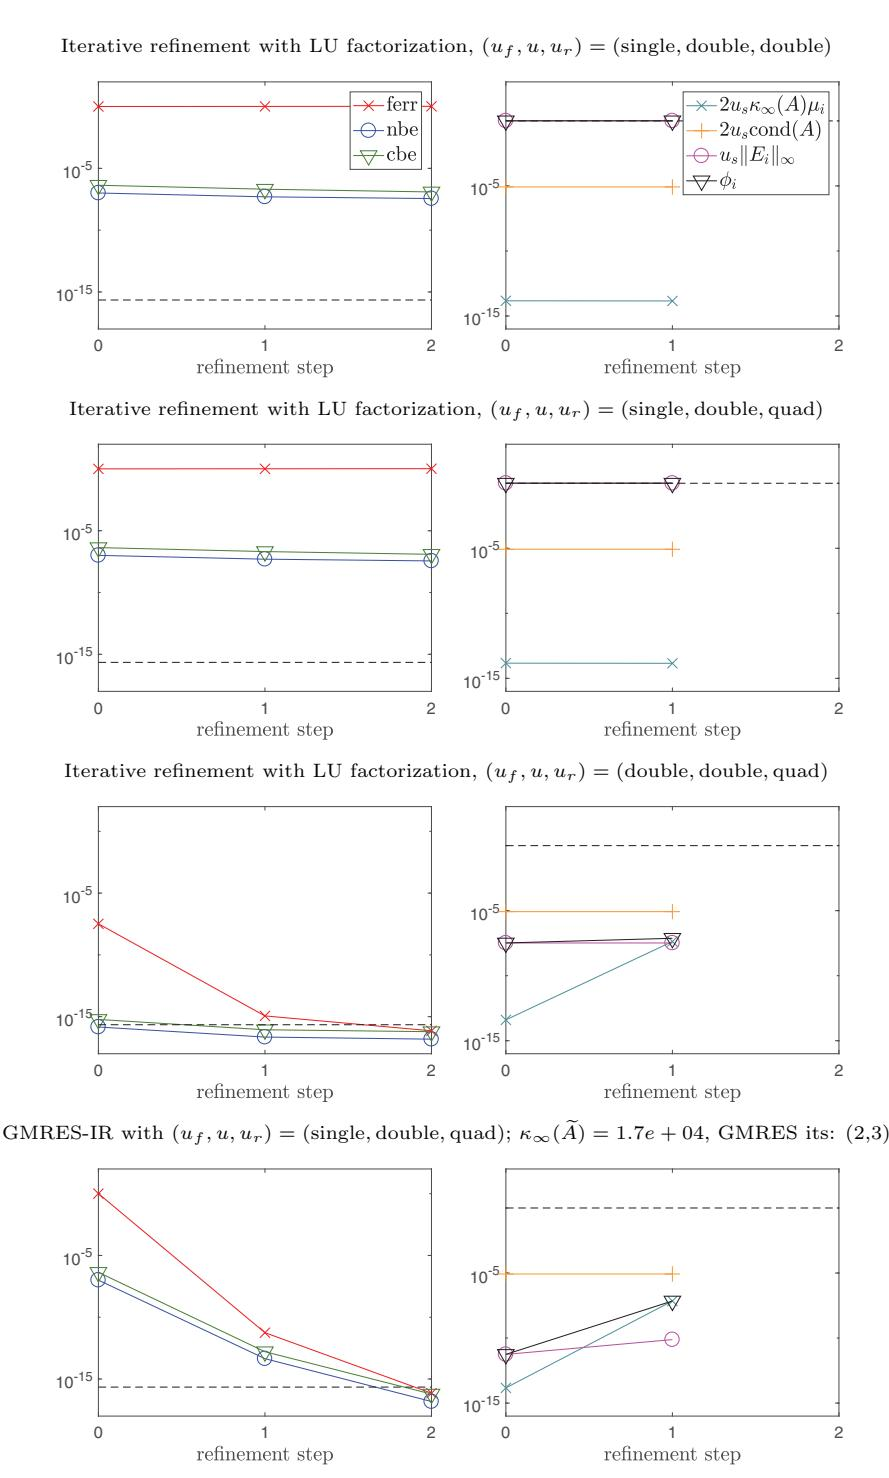
\includegraphics[width=\linewidth, height=0.8\textheight]{supplement/6bd513c5bfa16f6b36d4495fe15bf3b5a41cf109f9cd3e8095b57dd6c04b4baa.jpg}
    \end{column}
\end{columns}
\end{frame}


\section{Conclusion}


\begin{frame}[shrink=15]{Summary}
\setlength{\itemsep}{0pt}
\begin{block}{Unified Analysis of Iterative Refinement}
\small
We presented a general algorithm for solving $A x = b$ using three precisions:
\begin{itemize}
    \item \textbf{Working precision} $u$ (stores $A, b, x$)
    \item \textbf{Solver precision} $u_f$ (factorizes $A$)
    \item \textbf{Residual precision} $u_r$ (computes $r = b - A x$)
\end{itemize}
\end{block}

\begin{block}{Key Results}
\small
\begin{itemize}
    \item Derived rigorous forward and backward error bounds.
    \item Unified and generalized many existing rounding error analyses.
\end{itemize}
\end{block}

\begin{block}{Viability of Half-Precision}
\small
\begin{itemize}
    \item \textbf{LU Solver:} Solves to single precision accuracy for $\kappa_\infty(A) \leq 10^4$.
    \item \textbf{GMRES Solver:} Extends range to $\kappa_\infty(A) \leq 10^8$.
    \item The $O(n^3)$ factorization is performed entirely in half precision.
\end{itemize}
\end{block}
\end{frame}
\begin{frame}{Future Work}
    \begin{block}{Limitations and Future Directions}
The proposed method has specific scaling requirements and offers clear avenues for future research.
\end{block}

\begin{itemize}
    \item \textbf{Scaling Requirements:} Convergence is currently bounded by the condition number $\kappa_{\infty}(A)$.
    \item \textbf{Recursive Refinement:} Future work may explore recursive application of the algorithm to handle ill-conditioned systems.
    \item \textbf{Solver Diversity:} Analysis and implementation of different solvers (e.g., sparse or iterative) within the framework.
\end{itemize}
\end{frame}
\begin{frame}
    \centering
    \Huge \color{mathblue} Thank You!
\end{frame}\end{document}